%!TEX TS-program = pdflatex
%!TEX encoding = UTF-8 Unicode

\documentclass[11pt]{article}
\usepackage{jeffe,handout,graphicx,mathtools}
\usepackage[utf8x]{inputenc}			% allow Unicode in .tex file
\usepackage{enumerate}
\usepackage{fourier-orns}

\def\Sym#1{\texttt{\upshape\textcolor{BrickRed}{#1}}}
\def\SymBlue#1{\texttt{\upshape\textcolor{RoyalBlue}{#1}}}
\def\SymGreen#1{\texttt{\upshape\textcolor{PineGreen}{#1}}}
\def\_#1{\SymBlue{\underline{\smash{\textbf{#1}}}}}
\def\X#1{\SymGreen{$\overline{\textbf{#1}}$}}
\def\u#1{\raise0.5ex\hbox{\textcolor{RoyalBlue}{#1}}}

\def\Cdot{\mathbin{\text{\normalfont \textbullet}}}

\newcommand{\IsSinL}{\text{IsStringInL}}

% =========================================================
\begin{document}

\headers{CS/ECE 374}{Homework 7 (due March 29)}{Spring 2017}

\thispagestyle{empty}

\begin{center}
\Large\textbf{CS/ECE 374 \,\decosix\,  Spring 2017}%
\\
\LARGE\textbf{\decothreeleft~ Homework 7 ~\decothreeright}%
\\[0.5ex]
\large Due Wednesday, March 29, 2017 at 10am
\end{center}

\bigskip
\hrule
\bigskip

\noindent
\textbf{Groups of up to three people can submit joint solutions.}  Each problem should be submitted by exactly one person, and the beginning of the homework should clearly state the Gradescope names and email addresses of each group member.  In addition, whoever submits the homework must tell Gradescope who their other group members are.
\bigskip
\hrule
\bigskip


\noindent
The following unnumbered problems are not for submission or grading. 
No solutions for them will be provided but you can discuss them on Piazza.
\begin{itemize}
\item Consider a directed graph $G$, where each edge is colored either
  red, white, or blue. A walk in $G$ is called a {\em French flag
    walk} if its sequence of edge colors is red, white, blue, red,
  white, blue, and so on. More formally, a walk $v_0\rightarrow v_1
  \rightarrow \ldots \rightarrow v_k$ is a French flag walk if, for
  every integer $i$, the edge $v_i \rightarrow v_{i+1}$ is red if $i
  \mod 3 = 0$, white if $i \mod 3 = 1$, and blue if $i \mod 3 = 2$.
  Describe an efficient algorithm to find all vertices in a given
  edge-colored directed graph $G$ that can be reached from a given
  vertex $v$ through a French flag walk.
\item Describe a linear time algorithm that given a directed graph
  $G=(V,E)$ and a node $s \in V$ decides whether there is a cycle
  containing $s$. Do the same when $G$ is undirected.
\end{itemize}

\vspace{1cm}

\begin{enumerate}
%\parindent 1.5em \itemsep 3ex plus 0.5fil

%----------------------------------------------------------------------
%\def\arraystretch{1.2}

%----------------------------------------------------------------------
\item Let $G=(V,E)$ be directed graph. A subset of edges are colored
  red and a subset are colored blue and the rest are not colored.  Let
  $R \subset E$ be the set of red edges and $B \subset E$ be the set
  of blue edges.  Describe an efficient algorithm that given $G$ and
  two nodes $s,t \in V$ checks whether there is an $s$-$t$ path in $G$
  that contains at most one red edge and at most one blue edge. Ideally
  your algorithm should run in $O(n+m)$ time where $n = |V|$ and $m = |E|$.

%----------------------------------------------------------------------
\item The police department in the city of Shampoo-Banana has made all
  streets one-way. The mayor contends that there is still a way to
  drive legally from any intersection in the city to any other
  intersection, but the opposition is not convinced. The city needs an
  algorithm to check whether the mayor's contention is indeed true.
\begin{itemize}
\item Formulate this problem graph-theoretically, and
describe an efficent algorithm for it.
\item Suppose it turns out that the mayor’s original claim is
  false. Call an intersection $u$ {\em good} if any intersection $v$
  that you can reach from $u$ has the property that $u$ can be reached 
  from $v$. Now the mayor claims that over 95\% of the
  intersections are good.  Describe an efficient algorithm to verify
  her claim. Your algorithm should basically be able to find all the
  good intersections.
\end{itemize}
Ideally your algorithms for both parts should run in linear time. You will
receive partial credit for a polynomial-time algorithm.


%----------------------------------------------------------------------
\item Given an undirected connected graph $G=(V,E)$ an edge $(u,v)$ is
  called a cut edge or a bridge if removing it from $G$ results in
  two connected components (which means that $u$ is in one component
  and $v$ in the other). The goal in this problem is to design an efficient
  algorithm to find {\em all} the cut-edges of a graph.

  \begin{itemize}
  \item What are the cut-edges in the graph shown in the figure?
           \begin{center}
                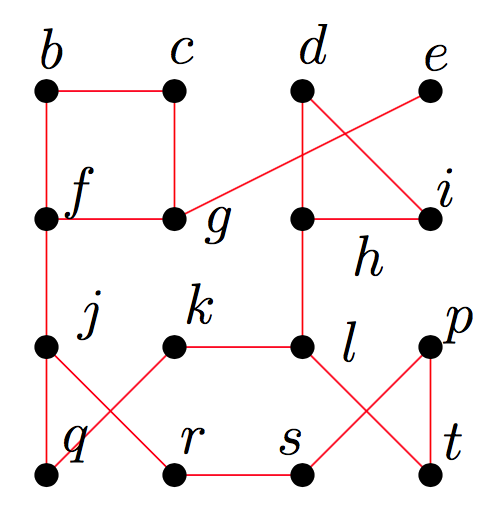
\includegraphics[width=5cm]{Fig/graph}
       \end{center}

  \item Given $G$ and edge $e=(u,v)$ describe a linear-time algorithm
    that checks whether $e$ is a cut-edge or not. What is the running time
    to find all cut-edges by trying your algorithm for each edge? No proofs
    necessary for this part.
  \item Consider {\em any} spanning tree $T$ for $G$. Prove that every
    cut-edge must belong to $T$. Conclude that there can be at most $(n-1)$
    cut-edges in a given graph. How does this information improve the 
    algorithm to find all cut-edges from the one in the previous step?
  \item Suppose $T$ is a spanning tree of $G$ rooted at $r$.
    Prove that an edge $(u,v)$ in $T$ where $u$ is
    the parent of $v$ is a cut-edge iff there is no edge in $G$, other
    than $(u,v)$, 
    with one end point in $T_v$ (sub-tree of $T$ rooted at $v$)
    and one end point outside $T_v$.
  \item Use the property in the preceding part to design a linear-time
    algorithm that outputs all the cut-edges of $G$. You don't have to 
    prove the correctness of the algorithm but you should point out how
    your algorithm ensures the desired property. {\em Hint:} Consider
    a DFS tree $T$ and some additional information you can compute
    during DFS. You may want to run DFS on the example graph with the
    cut edges identified.
  \end{itemize}


\end{enumerate}
%---------------------------------------
\vspace{1in}

\subsection*{Solved Problem}


\begin{enumerate}\parindent 1.5em
\setcounter{enumi}{3}

% ----------------------------------------------------------------------
\item

Professor McClane takes you out to a lake and hands you three empty jars.  Each jar holds a positive integer number of gallons; the capacities of the three jars may or may not be different.  The professor then demands that you put exactly $k$ gallons of water into one of the jars (which one doesn’t matter), for some integer $k$, using only the following operations:
\begin{enumerate}
\item Fill a jar with water from the lake until the jar is full.
\item Empty a jar of water by pouring water into the lake.
\item Pour water from one jar to another, until either the first jar is empty or the second jar is full, whichever happens first. 
\end{enumerate}
For example, suppose your jars hold $6$, $10$, and $15$ gallons.  Then you can put $13$ gallons of water into the third jar in six steps:
\begin{itemize}\itemsep0pt
\item Fill the third jar from the lake.
\item Fill the first jar from the third jar.  (Now the third jar holds $9$ gallons.)
\item Empty the first jar into the lake.
\item Fill the second jar from the lake.
\item Fill the first jar from the second jar.  (Now the second jar holds $4$ gallons.)
\item Empty the second jar into the third jar.
\end{itemize}

Describe and analyze an efficient algorithm that either finds the smallest number of operations that leave exactly~$k$ gallons in any jar, or reports correctly that obtaining exactly~$k$ gallons of water is impossible.  Your input consists of the capacities of the three jars and the positive integer $k$.  For example, given the four numbers $6, 10, 15$ and $13$ as input, your algorithm should return the number $6$ (for the sequence of operations listed above).


\begin{solution}
Let $A,B,C$ denote the capacities of the three jars.  We reduce the problem to breadth-first search in the following directed graph:
\begin{itemize}
\item
$V = \Setbar{(a,b,c)\strut}{0\le a\le p \text{~and~} 0\le b\le B \text{~and~} 0 \le c\le C}$.  Each vertex corresponds to a possible \EMPH{configuration} of water in the three jars.  There are $(A+1)(B+1)(C+1) = O(ABC)$ vertices altogether.

\item
The graph has a directed edge $(a,b,c)\arcto(a’,b’c’)$ whenever it is possible to move from the first configuration to the second in one step.  Specifically, there is an edge from $(a,b,c)$ to each of the following vertices (except those already equal to $(a,b,c)$):
\begin{itemize}
\item $(0,b,c)$ and $(a,0,c)$ and $(a,b,0)$ — dumping a jar into the lake
\item $(A,b,c)$ and $(a,B,c)$ and $(a,b,C)$ — filling a jar from the lake
\item $\left.\begin{cases}
		(0, a+b, c) & \text{if $a+b\le B$}\\
		(a+b-B, B, c) & \text{if $a+b \ge B$}
	\end{cases}\right\}$ — pouring from the first jar into the second
\item $\left.\begin{cases}
		(0, b, a+c) & \text{if $a+c\le C$}\\
		(a+c-C, b, C) & \text{if $a+c \ge C$}
	\end{cases}\right\}$ — pouring from the first jar into the third
\item $\left.\begin{cases}
		(a+b, 0, c) & \text{if $a+b\le A$}\\
		(A, a+b-A, c) & \text{if $a+b \ge A$}
	\end{cases}\right\}$ — pouring from the second jar into the first
\item $\left.\begin{cases}
		(a, 0, b+c) & \text{if $b+c\le C$}\\
		(a, b+c-C, C) & \text{if $b+c \ge C$}
	\end{cases}\right\}$ — pouring from the second jar into the third
\item $\left.\begin{cases}
		(a+c, b, 0) & \text{if $a+c\le A$}\\
		(A, b, a+c-A) & \text{if $a+c \ge A$}
	\end{cases}\right\}$ — pouring from the third jar into the first
\item $\left.\begin{cases}
		(a, b+c, 0) & \text{if $b+c\le B$}\\
		(a, B, b+c-B) & \text{if $b+c \ge B$}
	\end{cases}\right\}$ — pouring from the third jar into the second
\end{itemize}
Since each vertex has at most 12 outgoing edges, there are at most $12(A+1)\*(B+1)(C+1) = O(ABC)$ edges altogether.
\end{itemize}

To solve the jars problem, we need to find the \EMPH{shortest path} in $G$ from the start vertex $(0,0,0)$ to any target vertex of the form $(k, \cdot, \cdot)$ or $(\cdot, k, \cdot)$ or $(\cdot,\cdot, k)$.  We can compute this shortest path by calling \EMPH{breadth-first search} starting at $(0,0,0)$, and then examining every target vertex by brute force.  If BFS does not visit any target vertex, we report that no legal sequence of moves exists.  Otherwise, we find the target vertex closest to $(0,0,0)$ and trace its parent pointers back to $(0,0,0)$ to determine the shortest sequence of moves.  The resulting algorithm runs in $O(V+E) ={}$\EMPH{$O(ABC)$ time}.

We can make this algorithm faster by observing that every move either leaves at least one jar empty or leaves at least one jar full.  Thus, we only need vertices $(a,b,c)$ where either $a=0$ or $b=0$ or $c=0$ or $a=A$ or $b=B$ or $c=C$; no other vertices are reachable from $(0,0,0)$.  The number of non-redundant vertices and edges is $O(AB+BC+AC)$.  Thus, if we only construct and search the relevant portion of $G$, the algorithm runs in \EMPH{$O(AB+BC+AC)$ time}.
\end{solution}

\begin{rubric}[for graph reduction problems]
10 points:
\begin{itemize}\cramped
\item 2 for correct vertices
\item 2 for correct edges
\begin{itemize}\cramped
\item $\!\!\!$\textonehalf\ for forgetting “directed”
\end{itemize}
\item 2 for stating the correct problem (shortest paths)
\begin{itemize}\cramped
\item “Breadth-first search” is not a problem; it’s an algorithm.
\end{itemize}
\item 2 points for correctly applying the correct algorithm (breadth-first search)
\begin{itemize}\cramped
\item $\!\!\!1$ for using Dijkstra instead of BFS
\end{itemize}
\item 2 points for time analysis in terms of the input parameters.
\item Max 8 points for $O(ABC)$ time; scale partial credit
\end{itemize}
\end{rubric}


\end{enumerate}




\end{document}
